%% question-13.tex
%%

%% ==============================
\subsection{Modélisation explicite d'une instruction}
\label{sec:question13}
%% ==============================

Le concept d'instruction est présenté à l'aide de la figure \ref{fig:instruction}. Une \emph{Instruction} peut être \emph{Skip} qui est une instruction pour passer son tour. Elle à 4 autres enfants qui sont \emph{Conditionnelle}, \emph{Iteration} (qui est composé
de plusieurs instructions), \emph{Affectation} et \emph{Action} qui est lié aux actions suivantes.

\begin{figure}[h!]
	\centering
	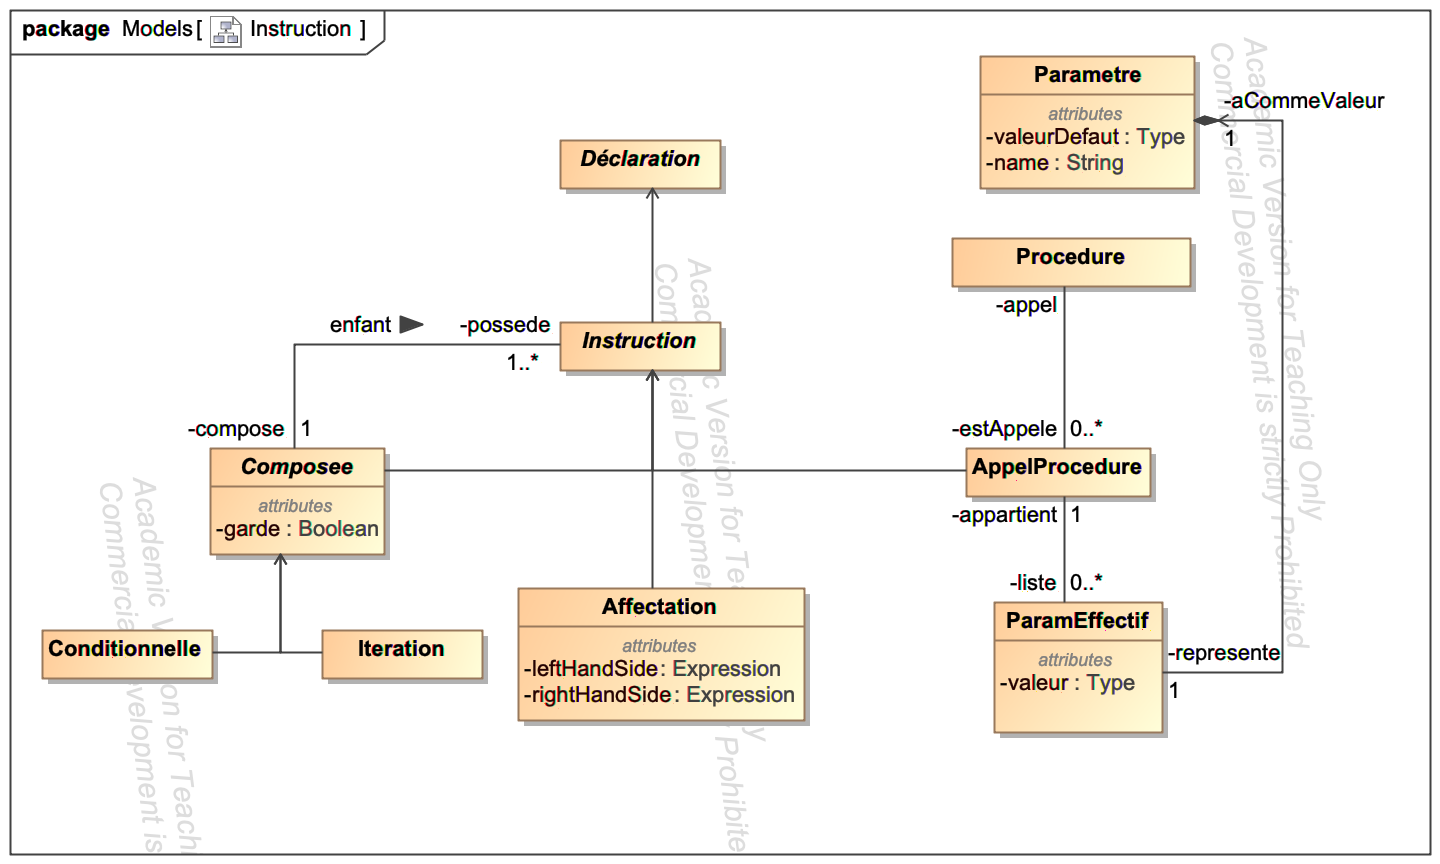
\includegraphics[width=450pt]{assets/class__Instruction}
	\caption{Diagramme de classe d'une instruction}
	\label{fig:instruction}
\end{figure}

\newpage